
\chapter{METHODOLOGY}
{\baselineskip=2\baselineskip

This chapter details the design and development of the automated eggplant sorting and grading system, following the Modified Waterfall SDLC model. Section 3.1 discusses the research design and procedural framework. Section 3.2 focuses on the hardware development, describing the design, architecture, and components essential of the conveyor and sorting mechanism. Section 3.3 explains the software development process, detailing the algorithms, tools, and models used for image processing, feature extraction, and classification. Section 3.4 elaborates on the system integration, illustrating how the hardware and software components interact to achieve seamless automation. Collectively, this chapter provides a comprehensive overview of the methods used to ensure the system's accuracy and reliability.


\section{Research Design}
Your research design.
\section{Formula}

\myequation{Some text}

\section{Tables}

\begin{center}
	\begin{longtable}{|l|l|l|}
		\caption{A sample long table.} \label{tab:long} \\
		
		\hline \multicolumn{1}{|c|}{\textbf{First column}} & \multicolumn{1}{c|}{\textbf{Second column}} & \multicolumn{1}{c|}{\textbf{Third column}} \\ \hline 
		\endfirsthead
		
		\multicolumn{3}{c}%
		{{\bfseries \tablename\ \thetable{} -- continued from previous page}} \\
		\hline \multicolumn{1}{|c|}{\textbf{First column}} & \multicolumn{1}{c|}{\textbf{Second column}} & \multicolumn{1}{c|}{\textbf{Third column}} \\ \hline 
		\endhead
		
		\hline \multicolumn{3}{|r|}{{Continued on next page}} \\ \hline
		\endfoot
		
		\hline \hline
		\endlastfoot
		
		One & abcdef ghjijklmn & 123.456778 \\
		One & abcdef ghjijklmn & 123.456778 \\
		One & abcdef ghjijklmn & 123.456778 \\
		One & abcdef ghjijklmn & 123.456778 \\
		One & abcdef ghjijklmn & 123.456778 \\
		One & abcdef ghjijklmn & 123.456778 \\
		One & abcdef ghjijklmn & 123.456778 \\
		One & abcdef ghjijklmn & 123.456778 \\
		One & abcdef ghjijklmn & 123.456778 \\
		One & abcdef ghjijklmn & 123.456778 \\
		One & abcdef ghjijklmn & 123.456778 \\
		One & abcdef ghjijklmn & 123.456778 \\
		One & abcdef ghjijklmn & 123.456778 \\
		One & abcdef ghjijklmn & 123.456778 \\
		One & abcdef ghjijklmn & 123.456778 \\
		One & abcdef ghjijklmn & 123.456778 \\
		One & abcdef ghjijklmn & 123.456778 \\
		One & abcdef ghjijklmn & 123.456778 \\
		One & abcdef ghjijklmn & 123.456778 \\
		One & abcdef ghjijklmn & 123.456778 \\
		One & abcdef ghjijklmn & 123.456778 \\
		One & abcdef ghjijklmn & 123.456778 \\
		One & abcdef ghjijklmn & 123.456778 \\
		One & abcdef ghjijklmn & 123.456778 \\
		One & abcdef ghjijklmn & 123.456778 \\
		One & abcdef ghjijklmn & 123.456778 \\
		One & abcdef ghjijklmn & 123.456778 \\
		One & abcdef ghjijklmn & 123.456778 \\
		One & abcdef ghjijklmn & 123.456778 \\
		One & abcdef ghjijklmn & 123.456778 \\
		One & abcdef ghjijklmn & 123.456778 \\
		One & abcdef ghjijklmn & 123.456778 \\
		One & abcdef ghjijklmn & 123.456778 \\
		One & abcdef ghjijklmn & 123.456778 \\
		One & abcdef ghjijklmn & 123.456778 \\
		One & abcdef ghjijklmn & 123.456778 \\
		One & abcdef ghjijklmn & 123.456778 \\
		One & abcdef ghjijklmn & 123.456778 \\
		One & abcdef ghjijklmn & 123.456778 \\
		One & abcdef ghjijklmn & 123.456778 \\
		One & abcdef ghjijklmn & 123.456778 \\
		One & abcdef ghjijklmn & 123.456778 \\
		One & abcdef ghjijklmn & 123.456778 \\
		One & abcdef ghjijklmn & 123.456778 \\
		One & abcdef ghjijklmn & 123.456778 \\
		One & abcdef ghjijklmn & 123.456778 \\
		One & abcdef ghjijklmn & 123.456778 \\
		One & abcdef ghjijklmn & 123.456778 \\
		One & abcdef ghjijklmn & 123.456778 \\
		One & abcdef ghjijklmn & 123.456778 \\
		One & abcdef ghjijklmn & 123.456778 \\
		One & abcdef ghjijklmn & 123.456778 \\
		One & abcdef ghjijklmn & 123.456778 \\
		One & abcdef ghjijklmn & 123.456778 \\
		One & abcdef ghjijklmn & 123.456778 \\
		One & abcdef ghjijklmn & 123.456778 \\
		One & abcdef ghjijklmn & 123.456778 \\
		One & abcdef ghjijklmn & 123.456778 \\
		One & abcdef ghjijklmn & 123.456778 \\
		One & abcdef ghjijklmn & 123.456778 \\
		One & abcdef ghjijklmn & 123.456778 \\
		One & abcdef ghjijklmn & 123.456778 \\
		One & abcdef ghjijklmn & 123.456778 \\
		One & abcdef ghjijklmn & 123.456778 \\
		One & abcdef ghjijklmn & 123.456778 \\
		One & abcdef ghjijklmn & 123.456778 \\
		One & abcdef ghjijklmn & 123.456778 \\
		One & abcdef ghjijklmn & 123.456778 \\
		One & abcdef ghjijklmn & 123.456778 \\
		One & abcdef ghjijklmn & 123.456778 \\
		One & abcdef ghjijklmn & 123.456778 \\
		One & abcdef ghjijklmn & 123.456778 \\
		One & abcdef ghjijklmn & 123.456778 \\
		One & abcdef ghjijklmn & 123.456778 \\
		One & abcdef ghjijklmn & 123.456778 \\
		One & abcdef ghjijklmn & 123.456778 \\
		One & abcdef ghjijklmn & 123.456778 \\
		One & abcdef ghjijklmn & 123.456778 \\
		One & abcdef ghjijklmn & 123.456778 \\
		One & abcdef ghjijklmn & 123.456778 \\
	\end{longtable}
\end{center}
\begin{table}[ht]
	\centering
	\caption{Sample Data Table}
	\label{tab:sample}
	\begin{tabular}{l c r}
		\toprule
		\textbf{Item} & \textbf{Quantity} & \textbf{Price (\$)} \\
		\midrule
		Apples & 10 & 0.50 \\
		Bananas & 5 & 0.30 \\
		Cherries & 20 & 1.20 \\
		Dates & 50 & 2.50 \\
		\bottomrule
	\end{tabular}
\end{table}
\section{Images}
\begin{figure}
	\centering
	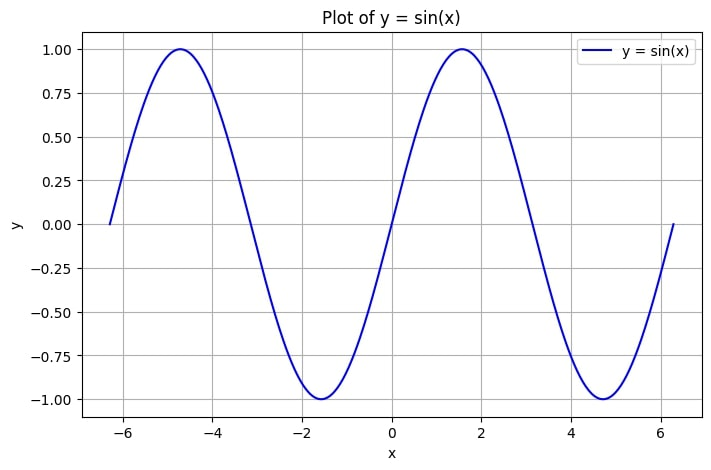
\includegraphics[width=0.7\linewidth]{figures/sinegraph}
	\caption{}
	\label{fig:sinegraph}
\end{figure}

\begin{figure}[h]
	\centering
	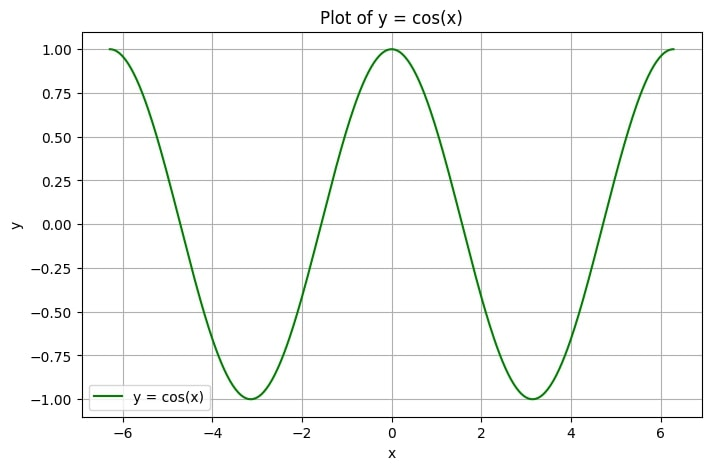
\includegraphics[height=0.3\textheight]{figures/cosinegraph}
	\caption[Cosine Graph]{Cosine Graph}
	\label{fig:cosinegraph}
\end{figure}
} 


